
\documentclass[template=tabling,81pt,headonall]{azmoon}
\usepackage{xepersian}
\usepackage{amsfonts}
\usepackage{graphicx}
\graphicspath{ {./images/} }
\settextfont{Yas}
\setdigitfont{A Iranian Sans}

\printanswers
    \teacher{محمد صالح علی اکبری}
    \teachertitle{دبیر}
    \city{گناباد}
    \schooltitle{متوسطه دوره دوم}
    \school{شهید رجایی}
    \grade{دهم}
    \branch{-}
    \topic{ریاضی}
    \examdate{02 شهریور 1402}
    \answertime{90 دقیقه}
    \begin{document}
	\begin{questions}
		\nointerlineskip%
		\vskip-\baselineskip
		\question[1.5]{%
در یک جمع 40 نفره 17 نفر با علی دوست هستند. همچنین 11 نفر با هیچ یک از علی و رضا دوست نیستند و 5 نفر با هر دو دوست هستند. چند نفر در این جمع فقط با رضا دوست هستند؟‌
\\‌
\\‌
\\}\question[1]{%
اگر $\tan\theta$ و $\sin\theta$ هم علامت باشند، آنگاه $\theta$ در کدام ربع مثلثاتی قرار دارد؟‌
\\‌
\\‌
\\}\question[1]{%
به کمک اتحاد حاصل عبارت زیر را حساب کنید. \begin {LTR} $999^2 =$ \\ \end{LTR}}\question[1.5]{%
اگر $\sqrt{x+2}+\sqrt{x-4} = 3$، حاصل عبارت $\sqrt{x+2}-\sqrt{x-4}$ را بدست آورید.‌
\\‌
\\‌
\\‌
\\‌
\\}\question[1]{%
عبارت رادیکالی زیر را به شکل توان گویا ساده کنید. \\ \begin{LTR} $\sqrt[4]{16}\times\sqrt[2]{9} = $ \end{LTR}}\question[1.5]{%
معادله زیر را حل کنید. \begin {LTR}$x^2+6x = 2$  \end{LTR}‌
\\}\question[0.5]{%
نا معادله زیر را حل کنید. \\ \begin{LTR} $|\dfrac{x-1}{2}-1| \geq 0$ \end{LTR}}\question[1]{%
نا معادله زیر را حل کنید. \\ \begin{LTR} $|\dfrac{x-1}{2}-1| \geq 3$ \end{LTR}‌
\\‌
\\‌
\\}\question[1.5]{%
نا معادله زیر را حل کنید. \\ \begin{LTR} $x+1 \leq 5-x < 2x +3$ \end{LTR}‌
\\‌
\\‌
\\‌
\\}\question[1]{%
یک تانکر گاز از یک استوانه و دو نیم کره به شعاع r در دو انتهای استوانه، تشکیل شده است. اگر ارتفاع استوانه ۳۰ متر باشد، حجم تانکر را بر حسب تابعی از r بنویسید.‌
\\‌
\\}\question[1]{%
مشخص کنید هر یک از متغیرهای زیر از نوع کدام دسته ترتیبی یا اسمی هستند؟
    \begin{parts}[1]\part{مراحل رشد یک انسان (نوزاد، کودک، نونهال، نوجوان، جوان، میان سال، کهن‌سال)}
\part{نژاد افراد (سفید پوست، زرد پوست، سیاه پوست)}
\part{رنگ موی افراد (مشکی، قهوه‌ای، طلایی)}
\part{کیفیت میوه هلو (درجه 1، درجه 2، درجه3)}
\end{parts}

    }\question[1.5]{%
از بین تعدادی کتاب مختلف می‌خواهیم سه کتاب را انتخاب کنیم و در قفسه‌ای بچینیم. اگر تعداد حالت‌های مختلف برای این کار ۲۱۰ تا باشد، تعداد کتاب‌ها چند تا است؟‌
\\‌
\\}\section{دانش‌ آموزان عزیز جهت کسب 6 نمره از سؤالات 13 تا 20 فقط ۳ سؤال را به دلخواه انتخاب و پاسخ دهید.}\question[2]{%
یک فروشگاه دو نوع کارت اعتباری A و B را می‌پذیرد. اگر 34 درصد از مشتریان کارت نوع A $(P(A) = \dfrac{34}{100})$ و 62 درصد کارت نوع B و 15 درصد هر دو کارت را همراه داشته باشند، چقدر احتمال دارد مشتریان با در اختیار داشتن حداقل یکی از این دو کارت از این فروشگاه خرید کنند؟‌
\\‌
\\‌
\\}\question[2]{%
یک آزمون چندگزینه‌ای شامل 10 سؤال 4 گزینه‌ای و 5 سؤال 2 گزینه‌ای (بله – خیر) است. فردی قصد دارد به سؤال‌‌ها به صورت تصادفی جواب دهد. او به چند روش می‌تواند این کار را انجام دهد اگر:
    \begin{parts}[1]\part{اگر مجبور باشد به همه سؤال‌ها جواب دهد؟}
\part{بتواند سؤال‌ها را بدون جواب هم بگذارد؟}
\end{parts}
‌
\\‌
\\
    }\question[2]{%
اگر A و B زیر مجموعه‌هایی از مجموعه مرجع باشند و در مورد تعداد اعضای مجموعه‌ها اطلاعات زیر را داشته باشیم:\\
$n(U)=100 ، n(A)=70 ، n(B) =30 ، n(A\bigcap B)=15$ \\
عبارت‌های زیر را حساب کنید.
    \begin{LTR}
        \begin{parts}[1]\part{$n(A\bigcap B^{\prime})= $}
\part{$n(A^{\prime}\bigcap B^{\prime}) =$}
\end{parts}
\end{LTR}
        
    }\question[2]{%
با فرض با معنی بودن هر کسر، درستی هر یک از تساوی‌های زیر را بررسی کنید.
    \begin{LTR}
        \begin{parts}[1]\part{$\dfrac{1}{\sin\theta}\times\tan\theta = \dfrac{1}{\cos\theta}$ \\ \\}
\part{$1-\dfrac{\cos^{2}x}{1+\sin x} = \sin x$}
\end{parts}
\end{LTR}
        ‌
\\‌
\\‌
\\
    }\question[2]{%
فرض کنید $\sin75^{\circ} \simeq 0.96$. مساحت مثلث ABC در شکل زیر را بدست آورید.
\\
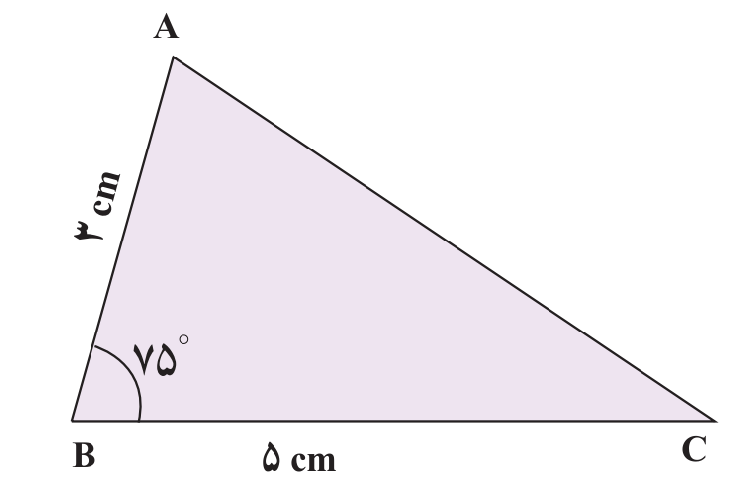
\includegraphics[scale = 0.3]{Screenshot_2023-08-23-14-40-21-311_cn.wps.moffice_eng}‌
\\‌
\\‌
\\}\question[2]{%
جدول تعیین علامت عبارت زیر را بنویسید. \begin {LTR} $x^2+6x-2$ \\ \\ \\ \\ \end{LTR}}\question[2]{%
تابع $f(x) = 3x-1$ را که دامنه آن مجموعه $\{\dfrac{1}{2},0,5\}$ است، رسم کنید. برد این تابع را به‌دست آورید و نمایش زوج مرتبی و نمودار پیکانی آن را ارائه دهید.‌
\\‌
\\‌
\\‌
\\‌
\\}\question[2]{%
نمودار تابع، یک سهمی است که از نقاط $(1 ، -2)$ و $(2، -3)$ می‌گذرد و محور yها را در نقطه‌ای به عرض ۱ قطع می‌کند. نمایش جبری این تابع را بیابید و نمودار آن را رسم و دامنه و برد تابع را مشخص کنید.‌
\\‌
\\‌
\\‌
\\‌
\\}\end{questions}
    \end{document}
    